\documentclass[12pt]{article}
\usepackage{natbib}
% \usepackage[hypertex]{hyperref}
\usepackage{bm}
\usepackage{amsfonts}
\usepackage{graphicx}


\oddsidemargin 0.0mm
\evensidemargin 0.0mm
\textwidth 160mm
\topmargin -10mm
\textheight 230mm
% \pagestyle{empty}

%%%%%%%%%%%%%%%%%%%%%%%%%%%%%%%%%%%%%%%%%%%%%%%%%%%%%%%%%%%%%%%%%%%

\newcommand{\threej}[6]
{ \left(\begin{array}{ccc}
#1&#2&#3\\
#4&#5&#6
\end{array}\right) }

\newcommand{\sixj}[6]
{ \left\{\begin{array}{ccc}
#1&#2&#3\\
#4&#5&#6
\end{array}\right\} }

\def\separation {0.5cm}
\def\ion#1#2  {#1\,{\small {#2}} }
\def\B{\textsc{BayesCLUMPY}}

%%%%%%%%%%%%%%%%%%%%%%%%%%%%%%%%%%%%%%%%%%%%%%%%%%%%%%%%%%%%%%%%%%%


% For generation of the HTML manual with tth:
% \def\tthdump#1{#1}      % For generating TeX source; ignored by tth
% Redefine symbols problematic for the browser:
%%tth:\def\ga{\hbox{$>\sim$}}
%%tth:\def\la{\hbox{$<\sim$}}
%%tth:\def\Mo{\hbox{$M_o$}}
%%tth:\def\Lo{\hbox{$L_o$}}
%%tth:\def\Mdot{\hbox{$M^{dot}$}}
%%tth:\def\Ivezic{Ivezic}

%%tth:\begin{html}<TITLE>User Manual for MOLPOP-CEP</TITLE>\end{html}
%%tth: This HTML file was generated from the TeX source by
%%tth: the translator TTH, which uses symbol fonts.  These fonts are
%%tth: not normally enabled for Netscape running under X, because of
%%tth: the way Netscape groups its fonts. If your browser has problems
%%tth: displaying the math symbols in this manual, an easy fix can be found
%%tth: on the TTH website at
%%tth:\begin{html}<A HREF="http://hutchinson.belmont.ma.us/tth/Xfonts.html">http://hutchinson.belmont.ma.us/tth/Xfonts.html</A>\end{html}
%%tth:\begin{html}<HR>\end{html}
%%%%%%%%%%%%%%%%%%%%%%%%%%%%%%%%%%%%%%%%%%%%%%%%%%%%%%%%%%%%%%%%%%%

\begin{document}

\title                  {\sc User Manual for \B\footnote{\B\ is one of the IAC computer
programs for synthesizing and making Bayesian inference of spectral energy distributions using the
clumpy dusty torus model of the Kentucky group.}}

\author{ A. Asensio Ramos \\ C. Ramos Almeida\\\\\\
         Instituto de Astrof\'{\i}sica de Canarias\\
         38205, La Laguna, Tenerife, Spain\\
        \\[0.5in] \today}
\date{}
\maketitle

\newpage

\tableofcontents

\newpage

\section*{Disclaimer}

This software is distributed ``as is'' and the authors do not take any responsability for
possible errors derived from its use by others. Apply it with care and
never trust the output without a careful meditation. \B\ can be freely used
provided that its origin is properly acknowledged and the references Asensio Ramos \& 
Ramos Almeida (2009; ApJ 696, 2075, 2013; MNRAS 428, 195) are cited and acknowledged in any
publication achieved with it. Before using \B\ we recommend the user to read carefully the
papers. Please, 
send us bug reports, comments and suggestions of possible improvements.
We point out that \B\ will be improved over the years, but it is now ready for a number of
interesting applications.

\section*{License}
\emph{This software is Copyright 2009 Andr\'es Asensio Ramos and Cristina Ramos Almeida. The software
may be used for experimental and research purposes only. Commercial use is
not permitted without prior agreement of the Copyright holders. The
software may be shared or distributed under the same restrictions, provided
all such users are made aware of this agreement. The software may not be
sold in whole or within part of a larger software product, whether in
source or binary forms.}

\newpage

%%%%%%%%%%%%%%%%%%%%%%%%%%%%%%%%%%%%%%%%%%%%%%%%%%
%%%%%%%%%%%%%%%%%%%%%%%%%%%%%%%%%%%%%%%%%%%%%%%%%%
\section{Introduction}

\B\ is a computer program that can be used for the fast synthesis of spectral
energy distributions (SED) emerging from clumpy dusty torus models developed by
the Kentucky group. The fast synthesis is accomplished by the usage
of machine learning tools that learn the database of models. These fast
synthesis capabilities are used in a Bayesian scheme for carrying out 
inference over the model parameters for observed SED. Inference can be carried out
with our own Monte Carlo sampler or the MultiNest sampler of Feroz, Hobson \& Bridges 
(2008, arXiv:0809.3437).
The code is written in standard Fortran 90 and IDL. A
front-end coded in IDL is given as a part of the 
distribution in order to facilitate a user-friendly execution of the program.

%%%%%%%%%%%%%%%%%%%%%%%%%%%%%%%%%%%%%%%%%%%%%%%%%%
%%%%%%%%%%%%%%%%%%%%%%%%%%%%%%%%%%%%%%%%%%%%%%%%%%
\section{Uncompressing and compiling \B}

The package comes in a single compressed file \texttt{bayesclumpy.tar.gz}. After
unpacking with \texttt{tar zxvf bayesclumpy.tar.gz}, the \B\ directory
will contain the following subdirectories:

\begin{enumerate}
\item
{\tt FORTRAN} contains the Fortran 90 sources and a makefile that can be used
to build the binary file.
\item
{\tt FILTERS} contains the spectral windows of all the possible filters included in \B. The
file The file {\tt normalizations.dat} in this directory indicates the names of the filters.
\item
{\tt NETWORKS} contains binary files with the weights of the neural networks. This directory is
essential for \B\ and its content should not be modified.
\item
{\tt OBSERVATIONS} is a container for all observed SEDs. An example file is given. 
\item
{\tt MARKOVCHAINS} is the default output directory for the Markov chains and for all the
results of the Bayesian inference.
\item
{\tt MANUAL} contains this manual. 
\end{enumerate}

The code has been tested on Linux platforms using the Intel Fortran
Compiler (\texttt{ifort}) and the GNU \texttt{gfortran} compiler. The compilation 
of the F90 code (in directory \texttt{FORTRAN}) is performed
with the supplied \texttt{makefile}. It is quite simple and easy to modify, and
contains additional comments about compiling. The
default compiler is the \texttt{ifort}, although you can use any other
compiler through the variable \texttt{COMPILER}. Examples for \texttt{ifort}
and \texttt{gfortran} are given. Just uncommment the one you prefer both in the \texttt{makefile}
file in the \texttt{FORTRAN} directory and the \texttt{Makefile} file in the 
\texttt{FORTRAN/NESTED} directory.
In order to obtain the executable file, just type:
\begin{verbatim}
       make all
\end{verbatim}
in the directory \texttt{FORTRAN} of \B. After compiling and linking, the executable is copied to the root directory of
\B.

The generated object and module files can be cleaned typing:
\begin{verbatim}
       make clean
\end{verbatim}


\section{Graphical front-ends}
Although the code can be run in command line by modifying by hand the input file, 
\B\ contains also a user friendly front-ends (GUI) for the simple execution and
analysis of the results. It is easily executed in IDL by entering:
\begin{verbatim}
IDL> .r bayesclumpy
IDL> bayesclumpy
\end{verbatim}
If errors appear when starting the GUI, use \texttt{bayesclumpy,/reset}.

\begin{figure}[!t]
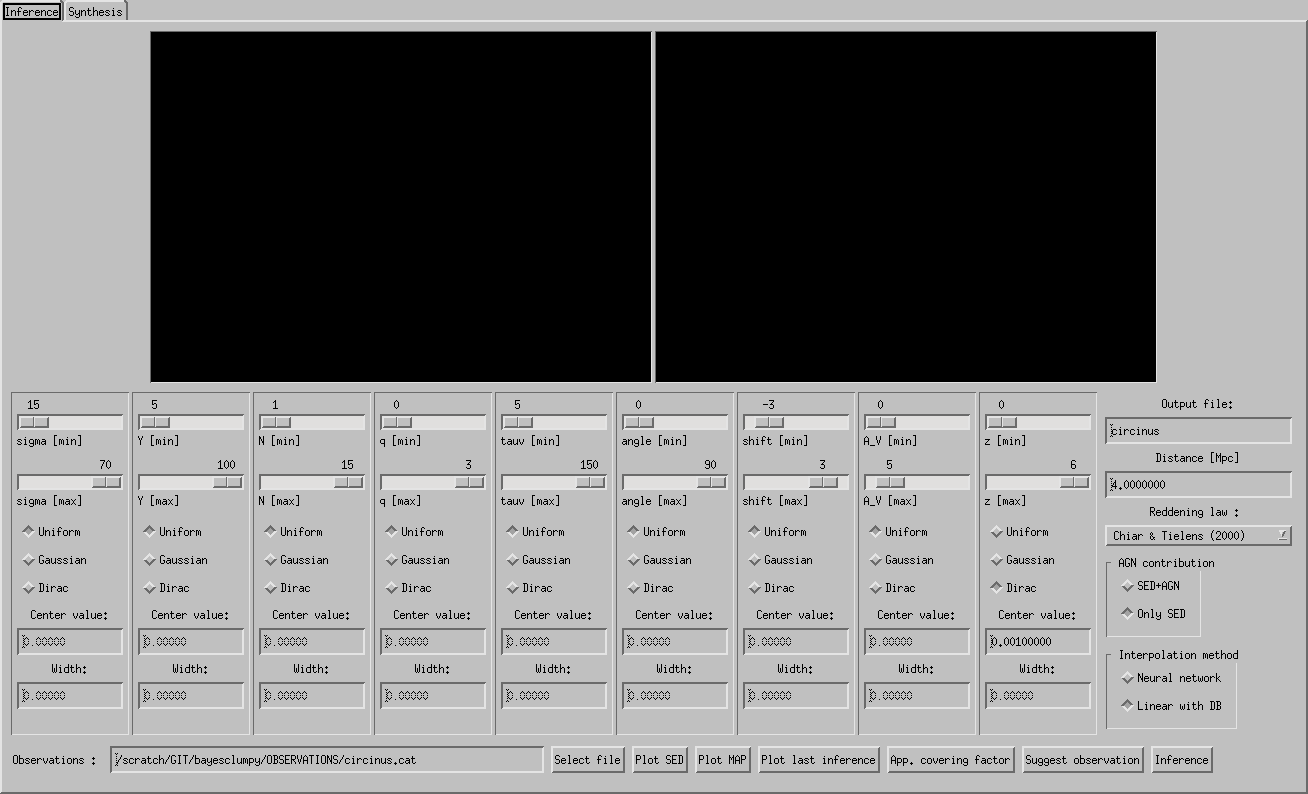
\includegraphics[scale=0.5]{snapshot1.png}
\caption{Screen dump of the graphical front-end used for the inference.
\label{fig:inversion_GUI}}
\end{figure}

\subsection{Inference}
This is the default tab when running the GUI. A snapshot is shown in Fig. \ref{fig:inversion_GUI}.
It can be used to visually change the
parameters defined for the inference and execute the inference. The available options are:
\begin{itemize}
\item Select file: opens a dialog box to select the catalog with the observations, as described in Section \ref{sec:observations}.
\item Plot SED: plots the selected SED for visualization purposes
\item Plot MAP: plots the observed SED, together with the best fit (MAP), the median and the 1$\sigma$ confidence region.
\item Plot last inference: plots the Markov chains and the ensuing marginal posteriors
\item App. covering factor: plots the posterior for the covering factor. Do not forget to enter the distance
 in Mpc because this quantity is used during the calculation
\item Suggest observation: use the Bayesian decision theory to suggest a new optimal filter (Asensio Ramos \& Ramos Almeida 2012)
\item Inference: run the Bayesian inference
\item Prior definition boxes. Allows to select the range of variation for each parameter and the shape of the prior (uniform, Gaussian or
Dirac). If you use a Dirac prior, enter the value in the ``Central value'' box. If you use a Gaussian prior, enter both the central
value and the width.
\item Output file: defines the root for all the output files on the inference. It will be saved in the \texttt{MARKOVCHAINS} directory
\item Distance: distance in Mpc to the source
\item Reddening law: select among the possible reddening laws. If other than ``No reddening'' is selected, fill the
information in the prior definition box for the extinction. We recommend to use extinction when there is an observed
evidence for it. Selecting a wide range of extinction can lead to multi-modal posteriors.
\item AGN contribution: use ``SED+AGN'' for AGN with broad lines and ``Only SED'' for Type-2 AGN
\item Interpolation method: used to select between the neural network interpolation or a multilinear
interpolation in the full database. In principle, we suggest the linear interpolation.
\end{itemize}


\begin{figure}[!t]
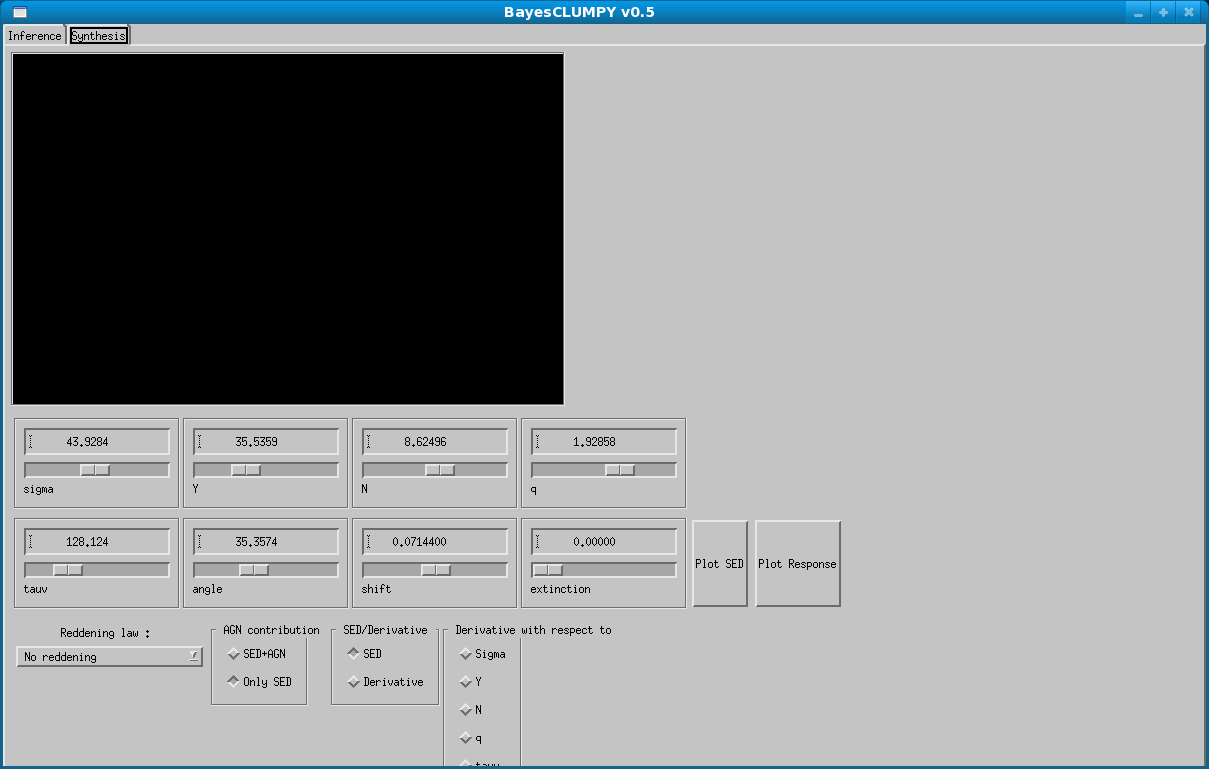
\includegraphics[scale=0.5]{snapshot2.png}
\caption{Screen dump of the graphical front-end used for the synthesis.
\label{fig:synthesis_GUI}}
\end{figure}

\subsection{Synthesis}
This is the GUI that allows the user to synthesize SEDs for any combination of the model
parameters. It is also possible to see the behavior of the response functions (derivative
of the SED at each wavelength with respect to any parameter).

%%%%%%%%%%%%%%%%%%%%%%%%%%%%%%%%%%%%%%%%%%%%%%%%%%
%%%%%%%%%%%%%%%%%%%%%%%%%%%%%%%%%%%%%%%%%%%%%%%%%%
\section{Observations}
\label{sec:observations}
The observations are usually saved in the \texttt{OBSERVATIONS} directory. For example, the
file for Circinus reads:
\begin{verbatim}
'Circinus'
8  200
'nacoJ'         1.60    0.2     
'F160W'         4.77    0.7     
'nacoK'         19      1.9     
'naco2p42'      31      3.1     
'nacoLp'        380     38      
'nacoMp'        1900    190     
'trecsSi2'      5939    297     
'trecsQa'       14078   3520
'T-ReCS'
      7.93260      136.241      20.4361
      7.95480      145.111      21.7666
      7.97700      161.525      24.2288
      7.99920      140.983      21.1475
      8.02140      133.449      20.0174
      8.04360      141.806      21.2709
      8.06580      146.340      21.9510
......
\end{verbatim}

Line by line, the file contains:
\begin{itemize}
\item The first line defines the name of the galaxy for identification purposes. This
name is used when generating the plots stored in the \texttt{PLOTS} directory when
clicking on the ``Plot MAP'' button.
\item Defines the number of photometric points (first number, 8 in the example) and spectroscopic points (second number, 200 in the example).
\item Photometric data: each line contains the name of the filter (see file \texttt{FILTERS/normalizations.dat'} for
a list of available filters), the flux in mJy and the error in mJy.
\item Name of the instrument for spectroscopy
\item Spectroscopic data: wavelength in $\mu$m (first column), flux in mJy (second column) and the error in mJy (third column)
\end{itemize}
If there is no spectroscopy available, just put 0 in the number of spectroscopic points and leave the photometric information only.
It is possible to give detection limits by putting the flux in negative (the
absolute value is used in the code) and giving the confidence (0.68, 0.95, etc.) in the second
column.

%%%%%%%%%%%%%%%%%%%%%%%%%%%%%%%%%%%%%%%%%%%%%%%%%%
%%%%%%%%%%%%%%%%%%%%%%%%%%%%%%%%%%%%%%%%%%%%%%%%%%

\section{Command Line Usage}
\B\ is fundamentally controlled via the IDL graphic user interface. We strongly
recommend the use of the interface. However, if you are brave enough, it is
possible to control it to do inference through the command line
using the input file \texttt{chain.cfg}.

%%%%%%%%%%%%%%%%%%%%%%%%%%%%%%%%%%%%%%%%%%%%%%%%%
\subsection{\texttt{chain.cfg}}
This file is used to indicate the input parameters for the inference process
carried out using Markov chains if one wants to do it manually. Using the file
provided with the distribution in the present version of \B, we analyze one by one all the inputs.

\begin{verbatim}
# What to do?
2
\end{verbatim}
This indicates the process to do: 1) start a standard MCMC chain, 2) continue a previous chain and 3) do
MultiNest inference.

\begin{verbatim}
# Number of parameters
9
\end{verbatim}
Definition of the number of parameters over which we want to carry out inference. It should
be left to 9 and fix parameters using the priors explained below.

\begin{verbatim}
# Maximum number of iterations
60000
\end{verbatim}
Maximum number of iterations of the Markov chain. This number should be chosen small (around 20000-30000) for
test purposes but should be increased to a much larger number for the final results to produce
better mixed chains.

\begin{verbatim}
# Burn-in [%]
40.0000
\end{verbatim}
Percentage of the Markov chain that is discarded from the beginning to avoid
transients. The value of 40\% is probably too much and something between 20-30\% can be
more appropriate. However, given the speed of the calculation, it is possible to
discard such a large piece of the chain without too much problem.

\begin{verbatim}
# Type of chain (MCMC, SAMPL, PRIO)
'MCMC'
\end{verbatim}
Set to MCMC to carry out inference. Set it to PRIO if you want to sample the prior distribution
for comparing with the posterior distribution. This last option is of reduced interest when
using uniform priors but can be of interest when more complex priors are used.

\begin{verbatim}
# File with observations (only used if MCMC)
'OBSERVATIONS/ngc1386_bayesclumpy.cat'
\end{verbatim}
File with the observed SED.

\begin{verbatim}
# Output chain filename
'MARKOVCHAINS/test'
\end{verbatim}
Name of the output file. Several extensions are added for different outputs.

\begin{verbatim}
# SED (0) or SED+AGN (1)
0
\end{verbatim}
Flag that allows the user to include the spectrum of the AGN. It uses
the spectral shape of Rowan-Robinson (1995).

\begin{verbatim}
# Reddening law
0
\end{verbatim}
It is possible to use four different options at the moment:
\begin{itemize}
 \item 0: no reddening law
 \item 2: Seaton (1979) MW
 \item 3: Fitzpatrick (1986) LMC
 \item 5: Calzetti et al. (2000)
\end{itemize}

\begin{verbatim}
PRIOR INFORMATION
# Information (name, minimum, maximum, type, mu, sigma)
'sigma'  15.0000   75.0000  'U'  0.00000  0.00000
'Y'  5.00000   50.0000  'U'  15.0000  2.50000
'N'  1.00000   15.0000  'U'  0.00000  0.00000
'q'  0.00000   2.00000  'U'  0.00000  0.00000
'tauv'  10.0000   67.0000  'U'  0.00000  0.00000
'angle'  0.00000   90.0000  'U'  85.0000  2.00000
'shift'  0.00000   2.00000  'U'  0.00000  0.00000
'extinction'  0.00000   10.0000  'D'  0.00000  0.00000
'redshift'  0.00000   6.00000  'D'  0.00000  0.00000
\end{verbatim}
The previous lines indicate the name of the parameter and the prior distribution for 
each one. Each line for each parameter shows its minimum and maximum value, the type
of prior and two quantities related to special priors (they are ignored if the prior
does not need them). At the moment, it is possible to 
select between:
\begin{itemize}
 \item Uniform priors (U): the prior probability of the parameter is the same in the interval
   between the maximum and minimum and zero outside the interval.
 \item Dirac delta priors (D): the prior probability of the parameter is zero in all the
   points of the interval except for the point indicated by the additional parameter $\mu$.
   This is a cheap way of fixing parameters to known values.
 \item Gaussian priors (G): the prior probability of the parameter follows a Gaussian shape
   centered at $\mu$ and with standard deviation $\sigma$.
\end{itemize}

%%%%%%%%%%%%%%%%%%%%%%%%%%%%%%%%%%%%%%%%%%%%%%%%%
\subsection{Execution}
\label{sec:execution}
After the \texttt{chain.cfg} file is set, the code is run by invoking
\begin{verbatim}
./clumpy_mcmc
\end{verbatim}
After the code is executed, output files are generated. These files are discussed in the
next section. While running, the code prints some information about the estimated
value of the evidence and the number of samples. At the end, a summary of the
results is also printed:
\begin{scriptsize}
\begin{verbatim}
ln(Z):              -20.764838
Acceptance Rate:      0.275456
Replacements:             7699
Total Samples:           27950
ln(Z):              -20.546586
 ln(ev)=  -20.546585595300542      +/-  0.14854888592743931     
 Total Likelihood Evaluations:        27950
 Sampling finished. Exiting MultiNest
 Length of posterior samples :         2661
 Number of parameters :            9
sigma : E(x)=  65.9822 - MAP=  69.1687
1-sigma : -   4.3476  +   2.5574
2-sigma : -   9.7182  +   3.3246
Y : E(x)=  55.8599 - MAP=  43.2088
1-sigma : -  27.8117  +  24.8530
2-sigma : -  43.1969  +  36.3919
N : E(x)=  12.1321 - MAP=  10.5982
1-sigma : -   1.7716  +   1.6503
2-sigma : -   2.9365  +   2.3783
q : E(x)=   2.6603 - MAP=   2.8560
1-sigma : -   0.3334  +   0.2084
2-sigma : -   0.7346  +   0.2813
tauv : E(x)=  20.4411 - MAP=  18.7710
1-sigma : -   2.6045  +   3.0676
2-sigma : -   4.9776  +   6.3088
angle : E(x)=  58.3109 - MAP=  79.4059
1-sigma : -  18.1883  +  18.4340
2-sigma : -  31.9523  +  26.2992
shift : E(x)=   1.6600 - MAP=   1.6520
1-sigma : -   0.0535  +   0.0614
2-sigma : -   0.1007  +   0.1432
extinction : E(x)=   2.1245 - MAP=   1.6052
1-sigma : -   1.3121  +   1.5464
2-sigma : -   1.9056  +   2.4055
redshift : E(x)=   0.0010 - MAP=   0.0010
1-sigma : -   0.0000  +   0.0000
2-sigma : -   0.0000  +   0.0000
 Evidence, <ln L> and Kullback-Leibler divergence
 -0.20546585      -9.5367174      -9.3312511    
PLOTS/marginal_Circinus.ps created
PLOTS/chains_Circinus.ps created
MAP bolometric flux [erg*cm^-2*s^-1] :    3.9595846e-09
MAP bolometric flux with extinction [erg*cm^-2*s^-1] :    3.6616562e-09
Median bolometric flux [erg*cm^-2*s^-1] :    4.4065919e-09
Median bolometric flux with extinction [erg*cm^-2*s^-1] :    3.9741406e-09
Figure PLOTS/MAP_Circinus.ps created
\end{verbatim}
\end{scriptsize}


%%%%%%%%%%%%%%%%%%%%%%%%%%%%%%%%%%%%%%%%%%%%%%%%%
\subsection{Output files}
\label{sec:output}

Every run of the \B\ code generates several files with different extensions. The root
of each file is the one selected in the ``Output file'' box in the GUI or in the 
\texttt{chain.cfg} file. Of all the files generated, the following are the most interesting:
\begin{itemize}
 \item \texttt{.confidence}: this is a text file that contains information on the retrieved parameters.
 Each line contains the estimated marginal median value, together with the confidence interval at 68\%
 and 95\% confidence, with the lower limit before the upper limit. The last line contains the set of
 parameters that produce the largest value of the full posterior distribution (if all the parameters
 have a uniform prior, this set of parameters coincides with the ones retrieved with a standard 
 least-squares minimization)
 \item \texttt{.hist1D}: this is an ASCII file that contains the marginal posteriors for all the parameters. The 
 file \texttt{read\_marginal.pro} is an example of how to read it
 \item \texttt{.MAP}: contains the values of the parameters that give the largest posterior. This is equivalent to
 the least-squares solution (modified by the presence of the priors)
 \item \texttt{.post\_equal\_weights.dat}: this is an ASCII file containing all the samples from the posterior. The file
 \texttt{read\_samples.pro} shows how to read it
 \item \texttt{.SED\_samples}: contains the SEDs that correspond to the samples of the posteriors. The file \texttt{read\_seds.pro}
 shows how to read this file
 \item \texttt{.stats}: contains information about the solution. It is of interest if several modes are found
\end{itemize}

%%%%%%%%%%%%%%%%%%%%%%%%%%%%%%%%%%%%%%%%%%%%%%%%%%
%%%%%%%%%%%%%%%%%%%%%%%%%%%%%%%%%%%%%%%%%%%%%%%%%%

%%%%%%%%%%%%%%%%%%%%%%%%%%%%%%%%%%%%%%%%%%%%%%%%%%
%%%%%%%%%%%%%%%%%%%%%%%%%%%%%%%%%%%%%%%%%%%%%%%%%%
% \begin{figure}
% \includegraphics[width=\columnwidth]{f5.eps}
% \caption{Screen dump of the graphical front-end used for the synthesis.
% \label{fig:synthesis_GUI}}
% \end{figure}


\section{MultiNest License}

MultiNest v 2.7 is used in this version of \B. MultiNest has the following license agreement.

\emph{This software is Copyright 2009 Farhan Feroz and Mike Hobson. The software
may be used for experimental and research purposes only. Commercial use is
not permitted without prior agreement of the Copyright holders. The
software may be shared or distributed under the same restrictions, provided
all such users are made aware of this agreement. The software may not be
sold in whole or within part of a larger software product, whether in
source or binary forms.}


\section*{Acknowledgements}
Finantial support by
the Spanish Ministry of Education and Science through projects AYA2007-63881, AYA2007-67965-C03-01,
the European Commission through the SOLAIRE network (MTRN-CT-2006-035484) and the
Spanish MEC under the Consolider-Ingenio 2010 Program grant CSD2006-00070 is gratefully acknowledged. 

% \bibliographystyle{apj}
% \bibliography{/home/aasensio/biblio}

\end{document}
